\documentclass[twoside]{book}

% Packages required by doxygen
\usepackage{fixltx2e}
\usepackage{calc}
\usepackage{doxygen}
\usepackage[export]{adjustbox} % also loads graphicx
\usepackage{graphicx}
\usepackage[utf8]{inputenc}
\usepackage{makeidx}
\usepackage{multicol}
\usepackage{multirow}
\PassOptionsToPackage{warn}{textcomp}
\usepackage{textcomp}
\usepackage[nointegrals]{wasysym}
\usepackage[table]{xcolor}

% Font selection
\usepackage[T1]{fontenc}
\usepackage[scaled=.90]{helvet}
\usepackage{courier}
\usepackage{amssymb}
\usepackage{sectsty}
\renewcommand{\familydefault}{\sfdefault}
\allsectionsfont{%
  \fontseries{bc}\selectfont%
  \color{darkgray}%
}
\renewcommand{\DoxyLabelFont}{%
  \fontseries{bc}\selectfont%
  \color{darkgray}%
}
\newcommand{\+}{\discretionary{\mbox{\scriptsize$\hookleftarrow$}}{}{}}

% Page & text layout
\usepackage{geometry}
\geometry{%
  a4paper,%
  top=2.5cm,%
  bottom=2.5cm,%
  left=2.5cm,%
  right=2.5cm%
}
\tolerance=750
\hfuzz=15pt
\hbadness=750
\setlength{\emergencystretch}{15pt}
\setlength{\parindent}{0cm}
\setlength{\parskip}{0.2cm}
\makeatletter
\renewcommand{\paragraph}{%
  \@startsection{paragraph}{4}{0ex}{-1.0ex}{1.0ex}{%
    \normalfont\normalsize\bfseries\SS@parafont%
  }%
}
\renewcommand{\subparagraph}{%
  \@startsection{subparagraph}{5}{0ex}{-1.0ex}{1.0ex}{%
    \normalfont\normalsize\bfseries\SS@subparafont%
  }%
}
\makeatother

% Headers & footers
\usepackage{fancyhdr}
\pagestyle{fancyplain}
\fancyhead[LE]{\fancyplain{}{\bfseries\thepage}}
\fancyhead[CE]{\fancyplain{}{}}
\fancyhead[RE]{\fancyplain{}{\bfseries\leftmark}}
\fancyhead[LO]{\fancyplain{}{\bfseries\rightmark}}
\fancyhead[CO]{\fancyplain{}{}}
\fancyhead[RO]{\fancyplain{}{\bfseries\thepage}}
\fancyfoot[LE]{\fancyplain{}{}}
\fancyfoot[CE]{\fancyplain{}{}}
\fancyfoot[RE]{\fancyplain{}{\bfseries\scriptsize Generated on Tue Aug 4 2015 16\+:37\+:54 for My Project by Doxygen }}
\fancyfoot[LO]{\fancyplain{}{\bfseries\scriptsize Generated on Tue Aug 4 2015 16\+:37\+:54 for My Project by Doxygen }}
\fancyfoot[CO]{\fancyplain{}{}}
\fancyfoot[RO]{\fancyplain{}{}}
\renewcommand{\footrulewidth}{0.4pt}
\renewcommand{\chaptermark}[1]{%
  \markboth{#1}{}%
}
\renewcommand{\sectionmark}[1]{%
  \markright{\thesection\ #1}%
}

% Indices & bibliography
\usepackage{natbib}
\usepackage[titles]{tocloft}
\setcounter{tocdepth}{3}
\setcounter{secnumdepth}{5}
\makeindex

% Hyperlinks (required, but should be loaded last)
\usepackage{ifpdf}
\ifpdf
  \usepackage[pdftex,pagebackref=true]{hyperref}
\else
  \usepackage[ps2pdf,pagebackref=true]{hyperref}
\fi
\hypersetup{%
  colorlinks=true,%
  linkcolor=blue,%
  citecolor=blue,%
  unicode%
}

% Custom commands
\newcommand{\clearemptydoublepage}{%
  \newpage{\pagestyle{empty}\cleardoublepage}%
}


%===== C O N T E N T S =====

\begin{document}

% Titlepage & ToC
\hypersetup{pageanchor=false,
             bookmarks=true,
             bookmarksnumbered=true,
             pdfencoding=unicode
            }
\pagenumbering{roman}
\begin{titlepage}
\vspace*{7cm}
\begin{center}%
{\Large My Project }\\
\vspace*{1cm}
{\large Generated by Doxygen 1.8.9.1}\\
\vspace*{0.5cm}
{\small Tue Aug 4 2015 16:37:54}\\
\end{center}
\end{titlepage}
\clearemptydoublepage
\tableofcontents
\clearemptydoublepage
\pagenumbering{arabic}
\hypersetup{pageanchor=true}

%--- Begin generated contents ---
\chapter{Hierarchical Index}
\section{Class Hierarchy}
This inheritance list is sorted roughly, but not completely, alphabetically\+:\begin{DoxyCompactList}
\item \contentsline{section}{Mecator\+Point}{\pageref{struct_mecator_point}}{}
\item N\+S\+Object\begin{DoxyCompactList}
\item \contentsline{section}{Baidu\+Pano\+Data}{\pageref{interface_baidu_pano_data}}{}
\begin{DoxyCompactList}
\item \contentsline{section}{Baidu\+Location\+Pano\+Data}{\pageref{interface_baidu_location_pano_data}}{}
\item \contentsline{section}{Baidu\+Poi\+Pano\+Data}{\pageref{interface_baidu_poi_pano_data}}{}
\end{DoxyCompactList}
\item \contentsline{section}{Baidu\+Pano\+Data\+Fetcher}{\pageref{interface_baidu_pano_data_fetcher}}{}
\item \contentsline{section}{Baidu\+Pano\+Overlay}{\pageref{interface_baidu_pano_overlay}}{}
\begin{DoxyCompactList}
\item \contentsline{section}{Baidu\+Pano\+Image\+Overlay}{\pageref{interface_baidu_pano_image_overlay}}{}
\item \contentsline{section}{Baidu\+Pano\+Label\+Overlay}{\pageref{interface_baidu_pano_label_overlay}}{}
\end{DoxyCompactList}
\item \contentsline{section}{Baidu\+Pano\+Utils}{\pageref{interface_baidu_pano_utils}}{}
\end{DoxyCompactList}
\item $<$N\+S\+Object$>$\begin{DoxyCompactList}
\item \contentsline{section}{$<$Baidu\+Panorama\+View\+Delegate$>$}{\pageref{protocol_baidu_panorama_view_delegate-p}}{}
\end{DoxyCompactList}
\item U\+I\+View\begin{DoxyCompactList}
\item \contentsline{section}{Baidu\+Panorama\+View}{\pageref{interface_baidu_panorama_view}}{}
\end{DoxyCompactList}
\end{DoxyCompactList}

\chapter{Class Index}
\section{Class List}
Here are the classes, structs, unions and interfaces with brief descriptions\+:\begin{DoxyCompactList}
\item\contentsline{section}{\hyperlink{interface_baidu_location_pano_data}{Baidu\+Location\+Pano\+Data} }{\pageref{interface_baidu_location_pano_data}}{}
\item\contentsline{section}{\hyperlink{interface_baidu_pano_data}{Baidu\+Pano\+Data} }{\pageref{interface_baidu_pano_data}}{}
\item\contentsline{section}{\hyperlink{interface_baidu_pano_data_fetcher}{Baidu\+Pano\+Data\+Fetcher} }{\pageref{interface_baidu_pano_data_fetcher}}{}
\item\contentsline{section}{\hyperlink{interface_baidu_pano_image_overlay}{Baidu\+Pano\+Image\+Overlay} }{\pageref{interface_baidu_pano_image_overlay}}{}
\item\contentsline{section}{\hyperlink{interface_baidu_pano_label_overlay}{Baidu\+Pano\+Label\+Overlay} }{\pageref{interface_baidu_pano_label_overlay}}{}
\item\contentsline{section}{\hyperlink{interface_baidu_pano_overlay}{Baidu\+Pano\+Overlay} }{\pageref{interface_baidu_pano_overlay}}{}
\item\contentsline{section}{\hyperlink{interface_baidu_panorama_view}{Baidu\+Panorama\+View} }{\pageref{interface_baidu_panorama_view}}{}
\item\contentsline{section}{\hyperlink{protocol_baidu_panorama_view_delegate-p}{$<$\+Baidu\+Panorama\+View\+Delegate$>$} }{\pageref{protocol_baidu_panorama_view_delegate-p}}{}
\item\contentsline{section}{\hyperlink{interface_baidu_pano_utils}{Baidu\+Pano\+Utils} }{\pageref{interface_baidu_pano_utils}}{}
\item\contentsline{section}{\hyperlink{interface_baidu_poi_pano_data}{Baidu\+Poi\+Pano\+Data} }{\pageref{interface_baidu_poi_pano_data}}{}
\item\contentsline{section}{\hyperlink{struct_mecator_point}{Mecator\+Point} }{\pageref{struct_mecator_point}}{}
\end{DoxyCompactList}

\chapter{Class Documentation}
\hypertarget{interface_baidu_location_pano_data}{}\section{Baidu\+Location\+Pano\+Data Class Reference}
\label{interface_baidu_location_pano_data}\index{Baidu\+Location\+Pano\+Data@{Baidu\+Location\+Pano\+Data}}
Inheritance diagram for Baidu\+Location\+Pano\+Data\+:\begin{figure}[H]
\begin{center}
\leavevmode
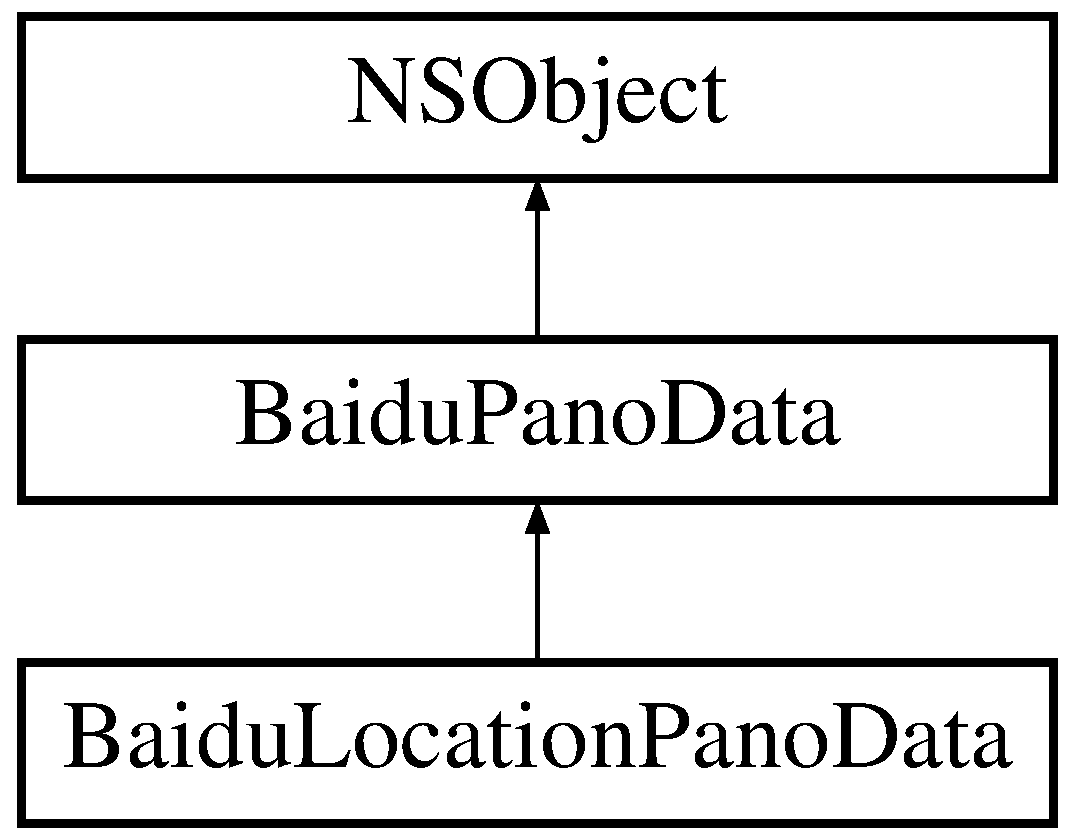
\includegraphics[height=3.000000cm]{interface_baidu_location_pano_data}
\end{center}
\end{figure}
\subsection*{Properties}
\begin{DoxyCompactItemize}
\item 
\hypertarget{interface_baidu_location_pano_data_a2c59bd88ac7a9f99847c41f6174654d2}{}N\+S\+String $\ast$ {\bfseries pid}\label{interface_baidu_location_pano_data_a2c59bd88ac7a9f99847c41f6174654d2}

\item 
\hypertarget{interface_baidu_location_pano_data_a94b2d368cb2467d4903c77fa55cb8574}{}N\+S\+String $\ast$ {\bfseries road\+Name}\label{interface_baidu_location_pano_data_a94b2d368cb2467d4903c77fa55cb8574}

\item 
\hypertarget{interface_baidu_location_pano_data_afc6bd63ea18ea362efa5c7eadee592e3}{}N\+S\+String $\ast$ {\bfseries mode}\label{interface_baidu_location_pano_data_afc6bd63ea18ea362efa5c7eadee592e3}

\end{DoxyCompactItemize}


The documentation for this class was generated from the following file\+:\begin{DoxyCompactItemize}
\item 
Baidu\+Location\+Pano\+Data.\+h\end{DoxyCompactItemize}

\hypertarget{interface_baidu_pano_data}{}\section{Baidu\+Pano\+Data Class Reference}
\label{interface_baidu_pano_data}\index{Baidu\+Pano\+Data@{Baidu\+Pano\+Data}}
Inheritance diagram for Baidu\+Pano\+Data\+:\begin{figure}[H]
\begin{center}
\leavevmode
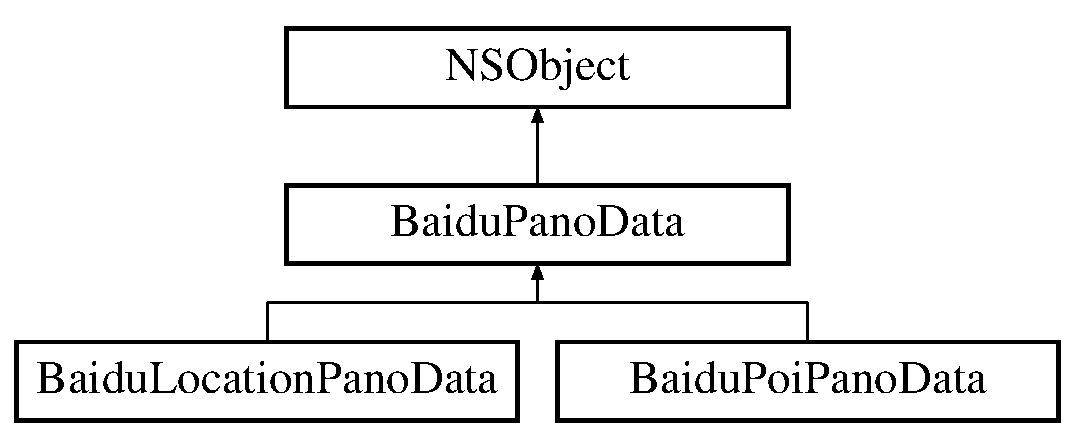
\includegraphics[height=3.000000cm]{interface_baidu_pano_data}
\end{center}
\end{figure}
\subsection*{Properties}
\begin{DoxyCompactItemize}
\item 
\hypertarget{interface_baidu_pano_data_a9b2b0a541dedae97020c705d05e57747}{}double {\bfseries x}\label{interface_baidu_pano_data_a9b2b0a541dedae97020c705d05e57747}

\item 
\hypertarget{interface_baidu_pano_data_a76ef908e3434e9d9a27d637cfdace2a2}{}double {\bfseries y}\label{interface_baidu_pano_data_a76ef908e3434e9d9a27d637cfdace2a2}

\item 
\hypertarget{interface_baidu_pano_data_ab18ba158af453b7083e2a08320da8c98}{}N\+S\+String $\ast$ {\bfseries type}\label{interface_baidu_pano_data_ab18ba158af453b7083e2a08320da8c98}

\item 
\hypertarget{interface_baidu_pano_data_a5d5be4b96ec81d950cd436032e37902e}{}N\+S\+String $\ast$ {\bfseries sdk\+Version}\label{interface_baidu_pano_data_a5d5be4b96ec81d950cd436032e37902e}

\item 
\hypertarget{interface_baidu_pano_data_ad7897e40c162c273b737074101fa8ead}{}int {\bfseries error\+Code}\label{interface_baidu_pano_data_ad7897e40c162c273b737074101fa8ead}

\item 
\hypertarget{interface_baidu_pano_data_a8a69f477f14610552d6457612e1c6a3a}{}N\+S\+String $\ast$ {\bfseries desc}\label{interface_baidu_pano_data_a8a69f477f14610552d6457612e1c6a3a}

\item 
\hypertarget{interface_baidu_pano_data_a4827cdb654418114403d803f29e3489a}{}B\+O\+O\+L {\bfseries has\+Panorama}\label{interface_baidu_pano_data_a4827cdb654418114403d803f29e3489a}

\end{DoxyCompactItemize}


The documentation for this class was generated from the following file\+:\begin{DoxyCompactItemize}
\item 
Baidu\+Pano\+Data.\+h\end{DoxyCompactItemize}

\hypertarget{interface_baidu_pano_data_fetcher}{}\section{Baidu\+Pano\+Data\+Fetcher Class Reference}
\label{interface_baidu_pano_data_fetcher}\index{Baidu\+Pano\+Data\+Fetcher@{Baidu\+Pano\+Data\+Fetcher}}
Inheritance diagram for Baidu\+Pano\+Data\+Fetcher\+:\begin{figure}[H]
\begin{center}
\leavevmode
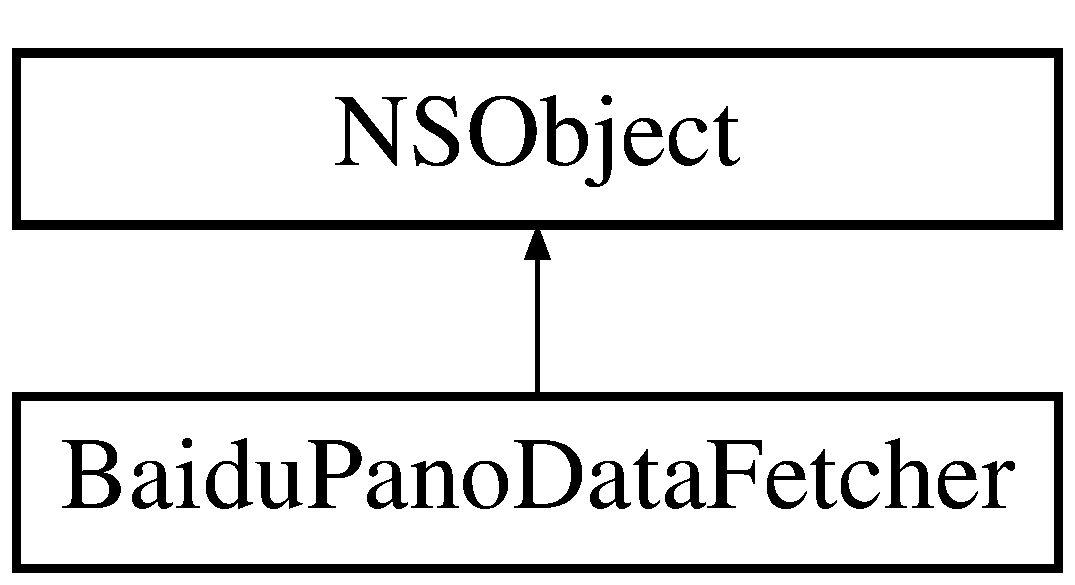
\includegraphics[height=2.000000cm]{interface_baidu_pano_data_fetcher}
\end{center}
\end{figure}
\subsection*{Class Methods}
\begin{DoxyCompactItemize}
\item 
(N\+S\+String $\ast$) + \hyperlink{interface_baidu_pano_data_fetcher_a984af94df4bdd13ecc4bf1bf2d7c9af9}{request\+Panorama\+Indoor\+Data\+With\+Iid\+:}
\item 
(N\+S\+String $\ast$) + \hyperlink{interface_baidu_pano_data_fetcher_a4df72f7368ecbeed658fbc0848ee0036}{request\+Panorama\+Recommendation\+Service\+Data\+With\+Pid\+:}
\item 
(\hyperlink{interface_baidu_poi_pano_data}{Baidu\+Poi\+Pano\+Data} $\ast$) + \hyperlink{interface_baidu_pano_data_fetcher_a24973faff16b705c6f5be43233af3550}{request\+Panorama\+Info\+With\+Uid\+:}
\item 
(\hyperlink{interface_baidu_location_pano_data}{Baidu\+Location\+Pano\+Data} $\ast$) + \hyperlink{interface_baidu_pano_data_fetcher_a399cac6672a5acc2571c751c8f6886a9}{request\+Panorama\+Info\+With\+X\+:\+Y\+:}
\item 
(\hyperlink{interface_baidu_location_pano_data}{Baidu\+Location\+Pano\+Data} $\ast$) + \hyperlink{interface_baidu_pano_data_fetcher_a13ba4cab3f69d9cd79aaad3ff0b81ec7}{request\+Panorama\+Info\+With\+Lon\+:\+Lat\+:}
\end{DoxyCompactItemize}


\subsection{Method Documentation}
\hypertarget{interface_baidu_pano_data_fetcher_a984af94df4bdd13ecc4bf1bf2d7c9af9}{}\index{Baidu\+Pano\+Data\+Fetcher@{Baidu\+Pano\+Data\+Fetcher}!request\+Panorama\+Indoor\+Data\+With\+Iid\+:@{request\+Panorama\+Indoor\+Data\+With\+Iid\+:}}
\index{request\+Panorama\+Indoor\+Data\+With\+Iid\+:@{request\+Panorama\+Indoor\+Data\+With\+Iid\+:}!Baidu\+Pano\+Data\+Fetcher@{Baidu\+Pano\+Data\+Fetcher}}
\subsubsection[{request\+Panorama\+Indoor\+Data\+With\+Iid\+:}]{\setlength{\rightskip}{0pt plus 5cm}+ (N\+S\+String $\ast$) request\+Panorama\+Indoor\+Data\+With\+Iid\+: 
\begin{DoxyParamCaption}
\item[{(N\+S\+String $\ast$)}]{iid}
\end{DoxyParamCaption}
}\label{interface_baidu_pano_data_fetcher_a984af94df4bdd13ecc4bf1bf2d7c9af9}
获取室内全景描述信息,其中包含室内相册相关信息,需要开发者自己解析 
\begin{DoxyParams}{Parameters}
{\em iid} & 室内信息的唯一\+I\+D,可以通过\+P\+O\+I查询获取到 \\
\hline
\end{DoxyParams}
\hypertarget{interface_baidu_pano_data_fetcher_a13ba4cab3f69d9cd79aaad3ff0b81ec7}{}\index{Baidu\+Pano\+Data\+Fetcher@{Baidu\+Pano\+Data\+Fetcher}!request\+Panorama\+Info\+With\+Lon\+:\+Lat\+:@{request\+Panorama\+Info\+With\+Lon\+:\+Lat\+:}}
\index{request\+Panorama\+Info\+With\+Lon\+:\+Lat\+:@{request\+Panorama\+Info\+With\+Lon\+:\+Lat\+:}!Baidu\+Pano\+Data\+Fetcher@{Baidu\+Pano\+Data\+Fetcher}}
\subsubsection[{request\+Panorama\+Info\+With\+Lon\+:\+Lat\+:}]{\setlength{\rightskip}{0pt plus 5cm}+ ({\bf Baidu\+Location\+Pano\+Data} $\ast$) request\+Panorama\+Info\+With\+Lon\+: 
\begin{DoxyParamCaption}
\item[{(double)}]{lon}
\item[{Lat:(double)}]{lat}
\end{DoxyParamCaption}
}\label{interface_baidu_pano_data_fetcher_a13ba4cab3f69d9cd79aaad3ff0b81ec7}
通过经纬度获取经纬度下全景相关信息,例如pid,全景类型等 
\begin{DoxyParams}{Parameters}
{\em pid} & \\
\hline
\end{DoxyParams}
\begin{DoxyReturn}{Returns}
json string 
\end{DoxyReturn}
\hypertarget{interface_baidu_pano_data_fetcher_a24973faff16b705c6f5be43233af3550}{}\index{Baidu\+Pano\+Data\+Fetcher@{Baidu\+Pano\+Data\+Fetcher}!request\+Panorama\+Info\+With\+Uid\+:@{request\+Panorama\+Info\+With\+Uid\+:}}
\index{request\+Panorama\+Info\+With\+Uid\+:@{request\+Panorama\+Info\+With\+Uid\+:}!Baidu\+Pano\+Data\+Fetcher@{Baidu\+Pano\+Data\+Fetcher}}
\subsubsection[{request\+Panorama\+Info\+With\+Uid\+:}]{\setlength{\rightskip}{0pt plus 5cm}+ ({\bf Baidu\+Poi\+Pano\+Data} $\ast$) request\+Panorama\+Info\+With\+Uid\+: 
\begin{DoxyParamCaption}
\item[{(N\+S\+String $\ast$)}]{uid}
\end{DoxyParamCaption}
}\label{interface_baidu_pano_data_fetcher_a24973faff16b705c6f5be43233af3550}
通过uid获取该poi下的全景描述信息,以此来判断此\+U\+I\+D下是否有全景 
\begin{DoxyParams}{Parameters}
{\em pid} & \\
\hline
\end{DoxyParams}
\begin{DoxyReturn}{Returns}
json string 
\end{DoxyReturn}
\hypertarget{interface_baidu_pano_data_fetcher_a399cac6672a5acc2571c751c8f6886a9}{}\index{Baidu\+Pano\+Data\+Fetcher@{Baidu\+Pano\+Data\+Fetcher}!request\+Panorama\+Info\+With\+X\+:\+Y\+:@{request\+Panorama\+Info\+With\+X\+:\+Y\+:}}
\index{request\+Panorama\+Info\+With\+X\+:\+Y\+:@{request\+Panorama\+Info\+With\+X\+:\+Y\+:}!Baidu\+Pano\+Data\+Fetcher@{Baidu\+Pano\+Data\+Fetcher}}
\subsubsection[{request\+Panorama\+Info\+With\+X\+:\+Y\+:}]{\setlength{\rightskip}{0pt plus 5cm}+ ({\bf Baidu\+Location\+Pano\+Data} $\ast$) request\+Panorama\+Info\+With\+X\+: 
\begin{DoxyParamCaption}
\item[{(double)}]{x}
\item[{Y:(double)}]{y}
\end{DoxyParamCaption}
}\label{interface_baidu_pano_data_fetcher_a399cac6672a5acc2571c751c8f6886a9}
通过墨卡托坐标获取坐标下全景的相关信息。 
\begin{DoxyParams}{Parameters}
{\em } & \\
\hline
\end{DoxyParams}
\hypertarget{interface_baidu_pano_data_fetcher_a4df72f7368ecbeed658fbc0848ee0036}{}\index{Baidu\+Pano\+Data\+Fetcher@{Baidu\+Pano\+Data\+Fetcher}!request\+Panorama\+Recommendation\+Service\+Data\+With\+Pid\+:@{request\+Panorama\+Recommendation\+Service\+Data\+With\+Pid\+:}}
\index{request\+Panorama\+Recommendation\+Service\+Data\+With\+Pid\+:@{request\+Panorama\+Recommendation\+Service\+Data\+With\+Pid\+:}!Baidu\+Pano\+Data\+Fetcher@{Baidu\+Pano\+Data\+Fetcher}}
\subsubsection[{request\+Panorama\+Recommendation\+Service\+Data\+With\+Pid\+:}]{\setlength{\rightskip}{0pt plus 5cm}+ (N\+S\+String $\ast$) request\+Panorama\+Recommendation\+Service\+Data\+With\+Pid\+: 
\begin{DoxyParamCaption}
\item[{(N\+S\+String $\ast$)}]{pid}
\end{DoxyParamCaption}
}\label{interface_baidu_pano_data_fetcher_a4df72f7368ecbeed658fbc0848ee0036}
获取某一个pid下对应的周边推荐信息 
\begin{DoxyParams}{Parameters}
{\em pid} & 全景pid \\
\hline
\end{DoxyParams}


The documentation for this class was generated from the following file\+:\begin{DoxyCompactItemize}
\item 
Baidu\+Pano\+Data\+Fetcher.\+h\end{DoxyCompactItemize}

\hypertarget{interface_baidu_pano_image_overlay}{}\section{Baidu\+Pano\+Image\+Overlay Class Reference}
\label{interface_baidu_pano_image_overlay}\index{Baidu\+Pano\+Image\+Overlay@{Baidu\+Pano\+Image\+Overlay}}
Inheritance diagram for Baidu\+Pano\+Image\+Overlay\+:\begin{figure}[H]
\begin{center}
\leavevmode
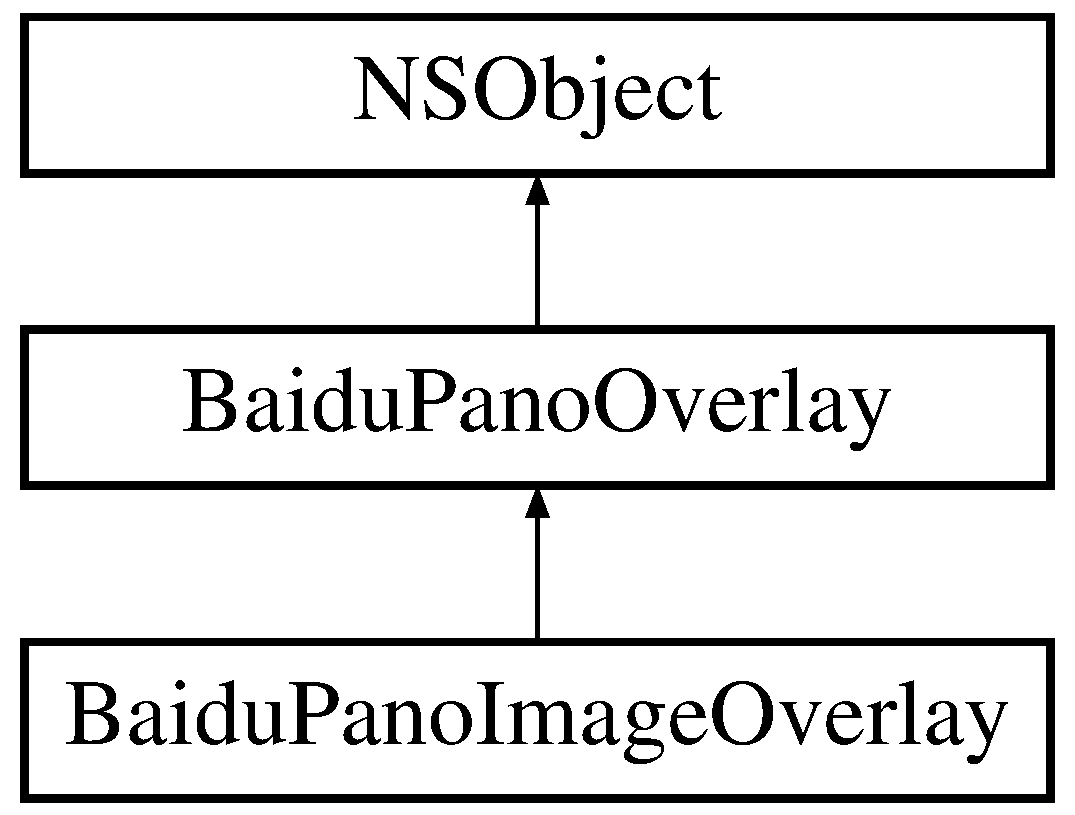
\includegraphics[height=3.000000cm]{interface_baidu_pano_image_overlay}
\end{center}
\end{figure}
\subsection*{Properties}
\begin{DoxyCompactItemize}
\item 
\hypertarget{interface_baidu_pano_image_overlay_ac35f2d117bb3368422a657d2d01fcf96}{}N\+S\+U\+R\+L $\ast$ {\bfseries url}\label{interface_baidu_pano_image_overlay_ac35f2d117bb3368422a657d2d01fcf96}

\item 
\hypertarget{interface_baidu_pano_image_overlay_a20b7c4d9c7c0e99953232f49bccbb266}{}C\+G\+Size {\bfseries size}\label{interface_baidu_pano_image_overlay_a20b7c4d9c7c0e99953232f49bccbb266}

\item 
\hypertarget{interface_baidu_pano_image_overlay_ab99543e78c3a3ab3b8eb0b102072efd5}{}U\+I\+Image $\ast$ {\bfseries image}\label{interface_baidu_pano_image_overlay_ab99543e78c3a3ab3b8eb0b102072efd5}

\end{DoxyCompactItemize}


The documentation for this class was generated from the following file\+:\begin{DoxyCompactItemize}
\item 
Baidu\+Pano\+Image\+Overlay.\+h\end{DoxyCompactItemize}

\hypertarget{interface_baidu_pano_label_overlay}{}\section{Baidu\+Pano\+Label\+Overlay Class Reference}
\label{interface_baidu_pano_label_overlay}\index{Baidu\+Pano\+Label\+Overlay@{Baidu\+Pano\+Label\+Overlay}}
Inheritance diagram for Baidu\+Pano\+Label\+Overlay\+:\begin{figure}[H]
\begin{center}
\leavevmode
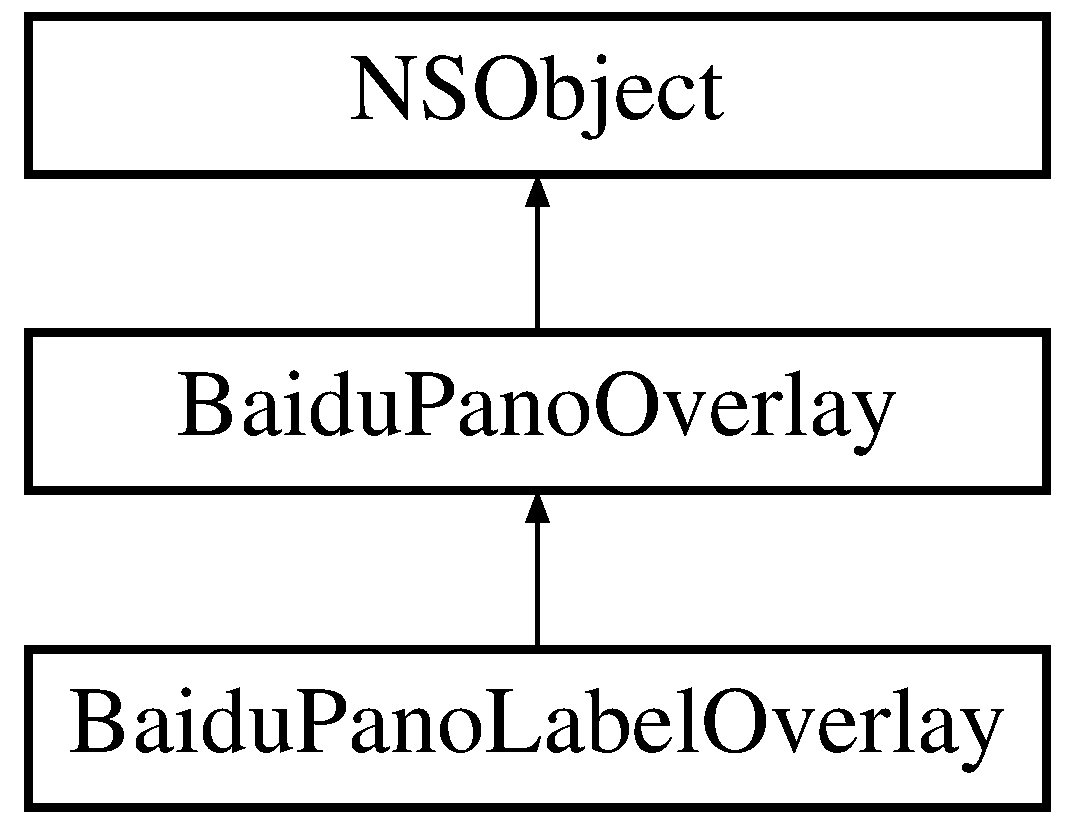
\includegraphics[height=3.000000cm]{interface_baidu_pano_label_overlay}
\end{center}
\end{figure}
\subsection*{Properties}
\begin{DoxyCompactItemize}
\item 
\hypertarget{interface_baidu_pano_label_overlay_ae67d5a9f1f79875a58c76434abfeeee5}{}N\+S\+String $\ast$ {\bfseries text}\label{interface_baidu_pano_label_overlay_ae67d5a9f1f79875a58c76434abfeeee5}

\item 
\hypertarget{interface_baidu_pano_label_overlay_a66d1d9ede9abbb14d758c945ca41a0d3}{}U\+I\+Color $\ast$ {\bfseries text\+Color}\label{interface_baidu_pano_label_overlay_a66d1d9ede9abbb14d758c945ca41a0d3}

\item 
\hypertarget{interface_baidu_pano_label_overlay_a8a13fbcb176af2fb528e8f19955d8559}{}U\+I\+Color $\ast$ {\bfseries background\+Color}\label{interface_baidu_pano_label_overlay_a8a13fbcb176af2fb528e8f19955d8559}

\item 
\hypertarget{interface_baidu_pano_label_overlay_a47f8018dc8a0579480c74f53e3209936}{}N\+S\+Integer {\bfseries font\+Size}\label{interface_baidu_pano_label_overlay_a47f8018dc8a0579480c74f53e3209936}

\item 
\hypertarget{interface_baidu_pano_label_overlay_a2dbf3e0ea55a94c1e7e90796ea27221e}{}U\+I\+Edge\+Insets {\bfseries edge\+Insets}\label{interface_baidu_pano_label_overlay_a2dbf3e0ea55a94c1e7e90796ea27221e}

\end{DoxyCompactItemize}


The documentation for this class was generated from the following file\+:\begin{DoxyCompactItemize}
\item 
Baidu\+Pano\+Label\+Overlay.\+h\end{DoxyCompactItemize}

\hypertarget{interface_baidu_pano_overlay}{}\section{Baidu\+Pano\+Overlay Class Reference}
\label{interface_baidu_pano_overlay}\index{Baidu\+Pano\+Overlay@{Baidu\+Pano\+Overlay}}
Inheritance diagram for Baidu\+Pano\+Overlay\+:\begin{figure}[H]
\begin{center}
\leavevmode
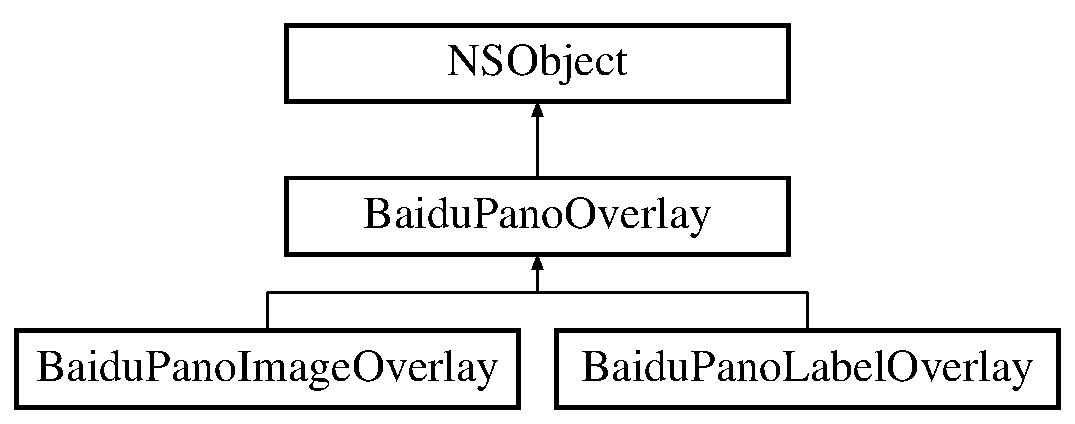
\includegraphics[height=3.000000cm]{interface_baidu_pano_overlay}
\end{center}
\end{figure}
\subsection*{Properties}
\begin{DoxyCompactItemize}
\item 
\hypertarget{interface_baidu_pano_overlay_a2c203a7fd4ebddb58214ca77dcbf1262}{}N\+S\+String $\ast$ {\bfseries overlay\+Key}\label{interface_baidu_pano_overlay_a2c203a7fd4ebddb58214ca77dcbf1262}

\item 
\hypertarget{interface_baidu_pano_overlay_a6ca1f3d09a958965c71dbc1240d3ab1a}{}Baidu\+Pano\+Overlay\+Type {\bfseries type}\label{interface_baidu_pano_overlay_a6ca1f3d09a958965c71dbc1240d3ab1a}

\item 
\hypertarget{interface_baidu_pano_overlay_a6bccfe66044e00ced701bdd7f6df6da8}{}C\+L\+Location\+Coordinate2\+D {\bfseries coordinate}\label{interface_baidu_pano_overlay_a6bccfe66044e00ced701bdd7f6df6da8}

\item 
\hypertarget{interface_baidu_pano_overlay_accb25227ffa324c593ea49bbae4a1505}{}double {\bfseries height}\label{interface_baidu_pano_overlay_accb25227ffa324c593ea49bbae4a1505}

\end{DoxyCompactItemize}


The documentation for this class was generated from the following file\+:\begin{DoxyCompactItemize}
\item 
Baidu\+Pano\+Overlay.\+h\end{DoxyCompactItemize}

\hypertarget{interface_baidu_panorama_view}{}\section{Baidu\+Panorama\+View Class Reference}
\label{interface_baidu_panorama_view}\index{Baidu\+Panorama\+View@{Baidu\+Panorama\+View}}
Inheritance diagram for Baidu\+Panorama\+View\+:\begin{figure}[H]
\begin{center}
\leavevmode
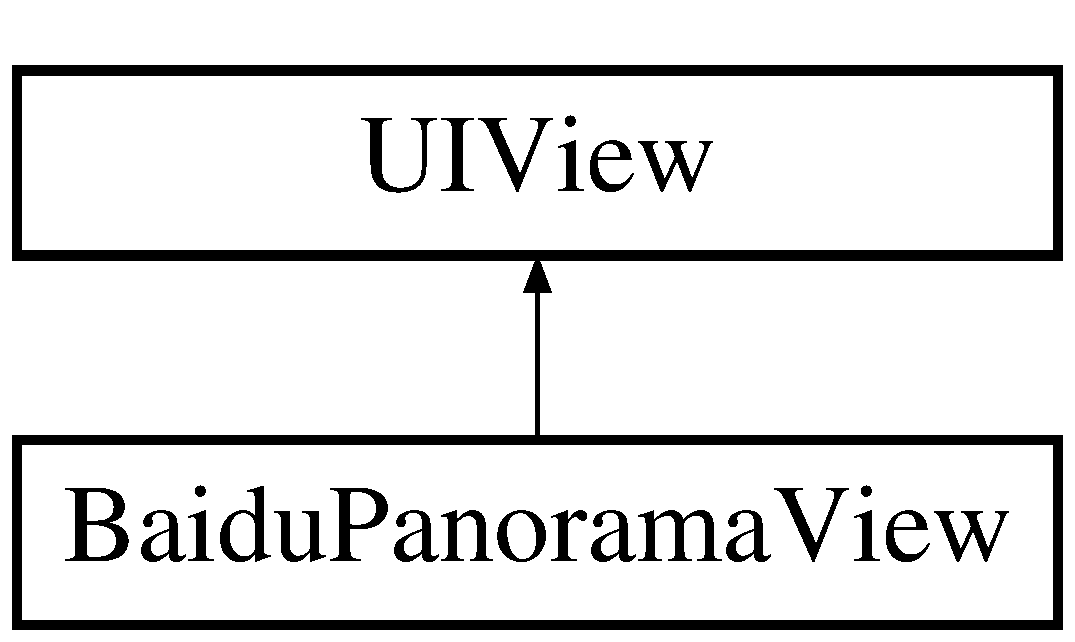
\includegraphics[height=2.000000cm]{interface_baidu_panorama_view}
\end{center}
\end{figure}
\subsection*{Instance Methods}
\begin{DoxyCompactItemize}
\item 
(id) -\/ \hyperlink{interface_baidu_panorama_view_a4d957cbad6a5ac3d913aa2f568f15e48}{init\+With\+Frame\+:key\+:}
\item 
(id) -\/ \hyperlink{interface_baidu_panorama_view_a6296448412d150d5e3c24f6fd7904fef}{init\+With\+Frame\+:}
\item 
(id) -\/ \hyperlink{interface_baidu_panorama_view_a64eae772265a972f0f2c6489243d2c4f}{init\+With\+Frame\+:mc\+X\+:mc\+Y\+:}
\item 
(void) -\/ \hyperlink{interface_baidu_panorama_view_af7206f937ec6fbc907eed36b8fa9ebce}{set\+Panorama\+With\+Pid\+:}
\item 
(void) -\/ \hyperlink{interface_baidu_panorama_view_a61b52d2ed24f7bf2d8e08a69cf16ce37}{set\+Panorama\+Access\+Key\+:}
\item 
(void) -\/ \hyperlink{interface_baidu_panorama_view_a6ed6dfcdeda2ee9b38645b90628591e8}{set\+Panorama\+With\+Lon\+:lat\+:}
\item 
(void) -\/ \hyperlink{interface_baidu_panorama_view_a6172e4a8b331b9e21f95db4ccd36afd4}{set\+Panorama\+With\+X\+:\+Y\+:}
\item 
(void) -\/ \hyperlink{interface_baidu_panorama_view_a339496b149bdd1d4d7b8852824f19df7}{set\+Panorama\+With\+Uid\+:}
\item 
(void) -\/ \hyperlink{interface_baidu_panorama_view_a23b03774273d83fb4c470a00f5b3ff63}{set\+Panorama\+With\+Uid\+:type\+:}
\item 
(void) -\/ \hyperlink{interface_baidu_panorama_view_ab24225239b38859fc66e92e9998213b4}{set\+Panorama\+Zoom\+Level\+:}
\item 
(void) -\/ \hyperlink{interface_baidu_panorama_view_ace6a54e7309447c11f6b9d42a93d827e}{set\+Panorama\+Image\+Level\+:}
\item 
(void) -\/ \hyperlink{interface_baidu_panorama_view_a11f799b9f91e66361f9125a65d7a6904}{set\+Panorama\+Pitch\+:}
\item 
(void) -\/ \hyperlink{interface_baidu_panorama_view_a11d516e6b3da9841779b3391de72bb1a}{set\+Panorama\+Heading\+:}
\item 
(void) -\/ \hyperlink{interface_baidu_panorama_view_a4614dac7c2d82742861e0849f73f900a}{set\+Direction\+Arrow\+Image\+:}
\item 
(void) -\/ \hyperlink{interface_baidu_panorama_view_aae8ed54ef190955aebe6653fbb082c55}{set\+Direction\+Arrow\+By\+Url\+:}
\item 
(void) -\/ \hyperlink{interface_baidu_panorama_view_ad404423fcbedbe17ae1847b7d06d77cc}{show\+Direction\+Arrow\+:}
\item 
(float) -\/ \hyperlink{interface_baidu_panorama_view_a12eb61616611c1c9e4947c026fb2cd59}{get\+Panorama\+Level}
\item 
(float) -\/ \hyperlink{interface_baidu_panorama_view_a29058d625d12c70ab5531f46ccee36e7}{get\+Panorama\+Pitch}
\item 
(float) -\/ \hyperlink{interface_baidu_panorama_view_af8634de5c37aa6a2b81ea161afed5b96}{get\+Panorama\+Heading}
\item 
(void) -\/ \hyperlink{interface_baidu_panorama_view_a1e534ac6f4342ed0ce7b6208387033f5}{add\+Overlay\+:}
\item 
(void) -\/ \hyperlink{interface_baidu_panorama_view_ae668b98f9036b7e50b0e7dc217fa8620}{remove\+Overlay\+:}
\item 
(void) -\/ \hyperlink{interface_baidu_panorama_view_af0d2fe0e5b5a7b67524b099d3cffcb83}{add\+Label\+Overlay\+By\+Id\+:coordinate\+:height\+:text\+:}
\item 
(void) -\/ \hyperlink{interface_baidu_panorama_view_ab851a3202611951265c474a226970f42}{add\+Image\+Overlay\+By\+Id\+:coordinate\+:height\+:image\+:}
\item 
(void) -\/ \hyperlink{interface_baidu_panorama_view_a372977bf92e0fddaa6693d95ffd5fb75}{add\+Label\+Overlay\+By\+Id\+:\+X\+:\+Y\+:\+Z\+:text\+:}
\item 
(void) -\/ \hyperlink{interface_baidu_panorama_view_ad8e1723b9122ffc20d7d719f630c4209}{add\+Image\+Overlay\+By\+Id\+:\+X\+:\+Y\+:\+Z\+:image\+:}
\end{DoxyCompactItemize}
\subsection*{Properties}
\begin{DoxyCompactItemize}
\item 
\hypertarget{interface_baidu_panorama_view_a630c3f630363be02283942719ea05e61}{}id$<$ \hyperlink{protocol_baidu_panorama_view_delegate-p}{Baidu\+Panorama\+View\+Delegate} $>$ {\bfseries delegate}\label{interface_baidu_panorama_view_a630c3f630363be02283942719ea05e61}

\end{DoxyCompactItemize}


\subsection{Method Documentation}
\hypertarget{interface_baidu_panorama_view_ab851a3202611951265c474a226970f42}{}\index{Baidu\+Panorama\+View@{Baidu\+Panorama\+View}!add\+Image\+Overlay\+By\+Id\+:coordinate\+:height\+:image\+:@{add\+Image\+Overlay\+By\+Id\+:coordinate\+:height\+:image\+:}}
\index{add\+Image\+Overlay\+By\+Id\+:coordinate\+:height\+:image\+:@{add\+Image\+Overlay\+By\+Id\+:coordinate\+:height\+:image\+:}!Baidu\+Panorama\+View@{Baidu\+Panorama\+View}}
\subsubsection[{add\+Image\+Overlay\+By\+Id\+:coordinate\+:height\+:image\+:}]{\setlength{\rightskip}{0pt plus 5cm}-\/ (void) add\+Image\+Overlay\+By\+Id\+: 
\begin{DoxyParamCaption}
\item[{(N\+S\+String $\ast$)}]{overlay\+Id}
\item[{coordinate:(C\+L\+Location\+Coordinate2\+D)}]{coor}
\item[{height:(double)}]{height}
\item[{image:(U\+I\+Image $\ast$)}]{image}
\end{DoxyParamCaption}
}\label{interface_baidu_panorama_view_ab851a3202611951265c474a226970f42}
添加图片覆盖物 
\begin{DoxyParams}{Parameters}
{\em overlayid} & 覆盖物id \\
\hline
{\em coordinate} & 经纬度坐标 \\
\hline
{\em height} & 覆盖物高度 \\
\hline
{\em image} & 覆盖物image \\
\hline
\end{DoxyParams}
\hypertarget{interface_baidu_panorama_view_ad8e1723b9122ffc20d7d719f630c4209}{}\index{Baidu\+Panorama\+View@{Baidu\+Panorama\+View}!add\+Image\+Overlay\+By\+Id\+:\+X\+:\+Y\+:\+Z\+:image\+:@{add\+Image\+Overlay\+By\+Id\+:\+X\+:\+Y\+:\+Z\+:image\+:}}
\index{add\+Image\+Overlay\+By\+Id\+:\+X\+:\+Y\+:\+Z\+:image\+:@{add\+Image\+Overlay\+By\+Id\+:\+X\+:\+Y\+:\+Z\+:image\+:}!Baidu\+Panorama\+View@{Baidu\+Panorama\+View}}
\subsubsection[{add\+Image\+Overlay\+By\+Id\+:\+X\+:\+Y\+:\+Z\+:image\+:}]{\setlength{\rightskip}{0pt plus 5cm}-\/ (void) add\+Image\+Overlay\+By\+Id\+: 
\begin{DoxyParamCaption}
\item[{(N\+S\+String $\ast$)}]{overlay\+Id}
\item[{X:(N\+S\+Integer)}]{x}
\item[{Y:(N\+S\+Integer)}]{y}
\item[{Z:(N\+S\+Integer)}]{z}
\item[{image:(U\+I\+Image $\ast$)}]{image}
\end{DoxyParamCaption}
}\label{interface_baidu_panorama_view_ad8e1723b9122ffc20d7d719f630c4209}
添加图片覆盖物 
\begin{DoxyParams}{Parameters}
{\em overlayid} & 覆盖物id \\
\hline
{\em x} & 墨卡托坐标x \\
\hline
{\em y} & 墨卡托坐标y \\
\hline
{\em z} & 覆盖物高度z \\
\hline
{\em image} & 显示的图片 \\
\hline
\end{DoxyParams}
\hypertarget{interface_baidu_panorama_view_af0d2fe0e5b5a7b67524b099d3cffcb83}{}\index{Baidu\+Panorama\+View@{Baidu\+Panorama\+View}!add\+Label\+Overlay\+By\+Id\+:coordinate\+:height\+:text\+:@{add\+Label\+Overlay\+By\+Id\+:coordinate\+:height\+:text\+:}}
\index{add\+Label\+Overlay\+By\+Id\+:coordinate\+:height\+:text\+:@{add\+Label\+Overlay\+By\+Id\+:coordinate\+:height\+:text\+:}!Baidu\+Panorama\+View@{Baidu\+Panorama\+View}}
\subsubsection[{add\+Label\+Overlay\+By\+Id\+:coordinate\+:height\+:text\+:}]{\setlength{\rightskip}{0pt plus 5cm}-\/ (void) add\+Label\+Overlay\+By\+Id\+: 
\begin{DoxyParamCaption}
\item[{(N\+S\+String $\ast$)}]{overlay\+Id}
\item[{coordinate:(C\+L\+Location\+Coordinate2\+D)}]{coor}
\item[{height:(double)}]{height}
\item[{text:(N\+S\+String $\ast$)}]{text}
\end{DoxyParamCaption}
}\label{interface_baidu_panorama_view_af0d2fe0e5b5a7b67524b099d3cffcb83}
添加文字覆盖物 
\begin{DoxyParams}{Parameters}
{\em overlayid} & 覆盖物id \\
\hline
{\em coordinate} & 经纬度坐标 \\
\hline
{\em height} & 覆盖物高度 \\
\hline
{\em text} & 显示的文字 \\
\hline
\end{DoxyParams}
\hypertarget{interface_baidu_panorama_view_a372977bf92e0fddaa6693d95ffd5fb75}{}\index{Baidu\+Panorama\+View@{Baidu\+Panorama\+View}!add\+Label\+Overlay\+By\+Id\+:\+X\+:\+Y\+:\+Z\+:text\+:@{add\+Label\+Overlay\+By\+Id\+:\+X\+:\+Y\+:\+Z\+:text\+:}}
\index{add\+Label\+Overlay\+By\+Id\+:\+X\+:\+Y\+:\+Z\+:text\+:@{add\+Label\+Overlay\+By\+Id\+:\+X\+:\+Y\+:\+Z\+:text\+:}!Baidu\+Panorama\+View@{Baidu\+Panorama\+View}}
\subsubsection[{add\+Label\+Overlay\+By\+Id\+:\+X\+:\+Y\+:\+Z\+:text\+:}]{\setlength{\rightskip}{0pt plus 5cm}-\/ (void) add\+Label\+Overlay\+By\+Id\+: 
\begin{DoxyParamCaption}
\item[{(N\+S\+String $\ast$)}]{overlay\+Id}
\item[{X:(N\+S\+Integer)}]{x}
\item[{Y:(N\+S\+Integer)}]{y}
\item[{Z:(N\+S\+Integer)}]{z}
\item[{text:(N\+S\+String $\ast$)}]{text}
\end{DoxyParamCaption}
}\label{interface_baidu_panorama_view_a372977bf92e0fddaa6693d95ffd5fb75}
添加文字覆盖物 
\begin{DoxyParams}{Parameters}
{\em overlayid} & 覆盖物id \\
\hline
{\em x} & 墨卡托坐标x \\
\hline
{\em y} & 墨卡托坐标y \\
\hline
{\em z} & 覆盖物高度z \\
\hline
{\em text} & 显示的文字 \\
\hline
\end{DoxyParams}
\hypertarget{interface_baidu_panorama_view_a1e534ac6f4342ed0ce7b6208387033f5}{}\index{Baidu\+Panorama\+View@{Baidu\+Panorama\+View}!add\+Overlay\+:@{add\+Overlay\+:}}
\index{add\+Overlay\+:@{add\+Overlay\+:}!Baidu\+Panorama\+View@{Baidu\+Panorama\+View}}
\subsubsection[{add\+Overlay\+:}]{\setlength{\rightskip}{0pt plus 5cm}-\/ (void) add\+Overlay\+: 
\begin{DoxyParamCaption}
\item[{({\bf Baidu\+Pano\+Overlay} $\ast$)}]{overlay}
\end{DoxyParamCaption}
}\label{interface_baidu_panorama_view_a1e534ac6f4342ed0ce7b6208387033f5}
添加覆盖物 
\begin{DoxyParams}{Parameters}
{\em overlay} & 抽象覆盖物 \\
\hline
\end{DoxyParams}
\hypertarget{interface_baidu_panorama_view_af8634de5c37aa6a2b81ea161afed5b96}{}\index{Baidu\+Panorama\+View@{Baidu\+Panorama\+View}!get\+Panorama\+Heading@{get\+Panorama\+Heading}}
\index{get\+Panorama\+Heading@{get\+Panorama\+Heading}!Baidu\+Panorama\+View@{Baidu\+Panorama\+View}}
\subsubsection[{get\+Panorama\+Heading}]{\setlength{\rightskip}{0pt plus 5cm}-\/ (float) get\+Panorama\+Heading 
\begin{DoxyParamCaption}
{}
\end{DoxyParamCaption}
}\label{interface_baidu_panorama_view_af8634de5c37aa6a2b81ea161afed5b96}
获取当前全景朝向 \hypertarget{interface_baidu_panorama_view_a12eb61616611c1c9e4947c026fb2cd59}{}\index{Baidu\+Panorama\+View@{Baidu\+Panorama\+View}!get\+Panorama\+Level@{get\+Panorama\+Level}}
\index{get\+Panorama\+Level@{get\+Panorama\+Level}!Baidu\+Panorama\+View@{Baidu\+Panorama\+View}}
\subsubsection[{get\+Panorama\+Level}]{\setlength{\rightskip}{0pt plus 5cm}-\/ (float) get\+Panorama\+Level 
\begin{DoxyParamCaption}
{}
\end{DoxyParamCaption}
}\label{interface_baidu_panorama_view_a12eb61616611c1c9e4947c026fb2cd59}
获取当前全景缩放级别 \hypertarget{interface_baidu_panorama_view_a29058d625d12c70ab5531f46ccee36e7}{}\index{Baidu\+Panorama\+View@{Baidu\+Panorama\+View}!get\+Panorama\+Pitch@{get\+Panorama\+Pitch}}
\index{get\+Panorama\+Pitch@{get\+Panorama\+Pitch}!Baidu\+Panorama\+View@{Baidu\+Panorama\+View}}
\subsubsection[{get\+Panorama\+Pitch}]{\setlength{\rightskip}{0pt plus 5cm}-\/ (float) get\+Panorama\+Pitch 
\begin{DoxyParamCaption}
{}
\end{DoxyParamCaption}
}\label{interface_baidu_panorama_view_a29058d625d12c70ab5531f46ccee36e7}
获取当前全景俯仰角 \hypertarget{interface_baidu_panorama_view_a6296448412d150d5e3c24f6fd7904fef}{}\index{Baidu\+Panorama\+View@{Baidu\+Panorama\+View}!init\+With\+Frame\+:@{init\+With\+Frame\+:}}
\index{init\+With\+Frame\+:@{init\+With\+Frame\+:}!Baidu\+Panorama\+View@{Baidu\+Panorama\+View}}
\subsubsection[{init\+With\+Frame\+:}]{\setlength{\rightskip}{0pt plus 5cm}-\/ (id) init\+With\+Frame\+: 
\begin{DoxyParamCaption}
\item[{(C\+G\+Rect)}]{frame}
\end{DoxyParamCaption}
}\label{interface_baidu_panorama_view_a6296448412d150d5e3c24f6fd7904fef}
全景视图初始化 
\begin{DoxyParams}{Parameters}
{\em frame} & 视图的frame \\
\hline
\end{DoxyParams}
\hypertarget{interface_baidu_panorama_view_a4d957cbad6a5ac3d913aa2f568f15e48}{}\index{Baidu\+Panorama\+View@{Baidu\+Panorama\+View}!init\+With\+Frame\+:key\+:@{init\+With\+Frame\+:key\+:}}
\index{init\+With\+Frame\+:key\+:@{init\+With\+Frame\+:key\+:}!Baidu\+Panorama\+View@{Baidu\+Panorama\+View}}
\subsubsection[{init\+With\+Frame\+:key\+:}]{\setlength{\rightskip}{0pt plus 5cm}-\/ (id) {\bf init\+With\+Frame\+:} 
\begin{DoxyParamCaption}
\item[{(C\+G\+Rect)}]{frame}
\item[{key:(N\+S\+String $\ast$)}]{key}
\end{DoxyParamCaption}
}\label{interface_baidu_panorama_view_a4d957cbad6a5ac3d913aa2f568f15e48}
全景视图初始化 
\begin{DoxyParams}{Parameters}
{\em frame} & 视图的frame \\
\hline
{\em key} & 百度\+L\+B\+S开放平台接入密钥 \\
\hline
\end{DoxyParams}
\hypertarget{interface_baidu_panorama_view_a64eae772265a972f0f2c6489243d2c4f}{}\index{Baidu\+Panorama\+View@{Baidu\+Panorama\+View}!init\+With\+Frame\+:mc\+X\+:mc\+Y\+:@{init\+With\+Frame\+:mc\+X\+:mc\+Y\+:}}
\index{init\+With\+Frame\+:mc\+X\+:mc\+Y\+:@{init\+With\+Frame\+:mc\+X\+:mc\+Y\+:}!Baidu\+Panorama\+View@{Baidu\+Panorama\+View}}
\subsubsection[{init\+With\+Frame\+:mc\+X\+:mc\+Y\+:}]{\setlength{\rightskip}{0pt plus 5cm}-\/ (id) {\bf init\+With\+Frame\+:} 
\begin{DoxyParamCaption}
\item[{(C\+G\+Rect)}]{frame}
\item[{mcX:(N\+S\+Integer)}]{x}
\item[{mcY:(N\+S\+Integer)}]{y}
\end{DoxyParamCaption}
}\label{interface_baidu_panorama_view_a64eae772265a972f0f2c6489243d2c4f}
全景视图初始化 
\begin{DoxyParams}{Parameters}
{\em frame} & 视图的frame \\
\hline
{\em mc\+X} & 百度墨卡托坐标x \\
\hline
{\em mc\+Y} & 百度墨卡托坐标y \\
\hline
\end{DoxyParams}
\hypertarget{interface_baidu_panorama_view_ae668b98f9036b7e50b0e7dc217fa8620}{}\index{Baidu\+Panorama\+View@{Baidu\+Panorama\+View}!remove\+Overlay\+:@{remove\+Overlay\+:}}
\index{remove\+Overlay\+:@{remove\+Overlay\+:}!Baidu\+Panorama\+View@{Baidu\+Panorama\+View}}
\subsubsection[{remove\+Overlay\+:}]{\setlength{\rightskip}{0pt plus 5cm}-\/ (void) remove\+Overlay\+: 
\begin{DoxyParamCaption}
\item[{(N\+S\+String $\ast$)}]{overlay\+Id}
\end{DoxyParamCaption}
}\label{interface_baidu_panorama_view_ae668b98f9036b7e50b0e7dc217fa8620}
移除覆盖物 
\begin{DoxyParams}{Parameters}
{\em overlay\+Id} & \\
\hline
\end{DoxyParams}
\hypertarget{interface_baidu_panorama_view_aae8ed54ef190955aebe6653fbb082c55}{}\index{Baidu\+Panorama\+View@{Baidu\+Panorama\+View}!set\+Direction\+Arrow\+By\+Url\+:@{set\+Direction\+Arrow\+By\+Url\+:}}
\index{set\+Direction\+Arrow\+By\+Url\+:@{set\+Direction\+Arrow\+By\+Url\+:}!Baidu\+Panorama\+View@{Baidu\+Panorama\+View}}
\subsubsection[{set\+Direction\+Arrow\+By\+Url\+:}]{\setlength{\rightskip}{0pt plus 5cm}-\/ (void) set\+Direction\+Arrow\+By\+Url\+: 
\begin{DoxyParamCaption}
\item[{(N\+S\+String $\ast$)}]{url}
\end{DoxyParamCaption}
}\label{interface_baidu_panorama_view_aae8ed54ef190955aebe6653fbb082c55}
设置道路箭头指引,通过image的url 
\begin{DoxyParams}{Parameters}
{\em url} & 图片资源url \\
\hline
\end{DoxyParams}
\hypertarget{interface_baidu_panorama_view_a4614dac7c2d82742861e0849f73f900a}{}\index{Baidu\+Panorama\+View@{Baidu\+Panorama\+View}!set\+Direction\+Arrow\+Image\+:@{set\+Direction\+Arrow\+Image\+:}}
\index{set\+Direction\+Arrow\+Image\+:@{set\+Direction\+Arrow\+Image\+:}!Baidu\+Panorama\+View@{Baidu\+Panorama\+View}}
\subsubsection[{set\+Direction\+Arrow\+Image\+:}]{\setlength{\rightskip}{0pt plus 5cm}-\/ (void) set\+Direction\+Arrow\+Image\+: 
\begin{DoxyParamCaption}
\item[{(U\+I\+Image $\ast$)}]{image}
\end{DoxyParamCaption}
}\label{interface_baidu_panorama_view_a4614dac7c2d82742861e0849f73f900a}
设置道路剪头image 
\begin{DoxyParams}{Parameters}
{\em image} & U\+I\+Image对象 \\
\hline
\end{DoxyParams}
\hypertarget{interface_baidu_panorama_view_a61b52d2ed24f7bf2d8e08a69cf16ce37}{}\index{Baidu\+Panorama\+View@{Baidu\+Panorama\+View}!set\+Panorama\+Access\+Key\+:@{set\+Panorama\+Access\+Key\+:}}
\index{set\+Panorama\+Access\+Key\+:@{set\+Panorama\+Access\+Key\+:}!Baidu\+Panorama\+View@{Baidu\+Panorama\+View}}
\subsubsection[{set\+Panorama\+Access\+Key\+:}]{\setlength{\rightskip}{0pt plus 5cm}-\/ (void) set\+Panorama\+Access\+Key\+: 
\begin{DoxyParamCaption}
\item[{(N\+S\+String $\ast$)}]{key}
\end{DoxyParamCaption}
}\label{interface_baidu_panorama_view_a61b52d2ed24f7bf2d8e08a69cf16ce37}
设定应用接入密钥 
\begin{DoxyParams}{Parameters}
{\em key} & 通过\+L\+B\+S开放平台创建应用获得 \\
\hline
\end{DoxyParams}
\hypertarget{interface_baidu_panorama_view_a11d516e6b3da9841779b3391de72bb1a}{}\index{Baidu\+Panorama\+View@{Baidu\+Panorama\+View}!set\+Panorama\+Heading\+:@{set\+Panorama\+Heading\+:}}
\index{set\+Panorama\+Heading\+:@{set\+Panorama\+Heading\+:}!Baidu\+Panorama\+View@{Baidu\+Panorama\+View}}
\subsubsection[{set\+Panorama\+Heading\+:}]{\setlength{\rightskip}{0pt plus 5cm}-\/ (void) set\+Panorama\+Heading\+: 
\begin{DoxyParamCaption}
\item[{(float)}]{heading}
\end{DoxyParamCaption}
}\label{interface_baidu_panorama_view_a11d516e6b3da9841779b3391de72bb1a}
设置全景图偏航角 
\begin{DoxyParams}{Parameters}
{\em heading} & 偏航角\+: 0$\sim$360 度 默认值\+: 0 度 \\
\hline
\end{DoxyParams}
\hypertarget{interface_baidu_panorama_view_ace6a54e7309447c11f6b9d42a93d827e}{}\index{Baidu\+Panorama\+View@{Baidu\+Panorama\+View}!set\+Panorama\+Image\+Level\+:@{set\+Panorama\+Image\+Level\+:}}
\index{set\+Panorama\+Image\+Level\+:@{set\+Panorama\+Image\+Level\+:}!Baidu\+Panorama\+View@{Baidu\+Panorama\+View}}
\subsubsection[{set\+Panorama\+Image\+Level\+:}]{\setlength{\rightskip}{0pt plus 5cm}-\/ (void) set\+Panorama\+Image\+Level\+: 
\begin{DoxyParamCaption}
\item[{(Image\+Definition)}]{image\+Definition}
\end{DoxyParamCaption}
}\label{interface_baidu_panorama_view_ace6a54e7309447c11f6b9d42a93d827e}
设置全景场景使用图片级别 
\begin{DoxyParams}{Parameters}
{\em level} & 图片级别 清晰度\+:\+Image\+Definition,默认值\+:middle \\
\hline
\end{DoxyParams}
\hypertarget{interface_baidu_panorama_view_a11f799b9f91e66361f9125a65d7a6904}{}\index{Baidu\+Panorama\+View@{Baidu\+Panorama\+View}!set\+Panorama\+Pitch\+:@{set\+Panorama\+Pitch\+:}}
\index{set\+Panorama\+Pitch\+:@{set\+Panorama\+Pitch\+:}!Baidu\+Panorama\+View@{Baidu\+Panorama\+View}}
\subsubsection[{set\+Panorama\+Pitch\+:}]{\setlength{\rightskip}{0pt plus 5cm}-\/ (void) set\+Panorama\+Pitch\+: 
\begin{DoxyParamCaption}
\item[{(float)}]{pitch}
\end{DoxyParamCaption}
}\label{interface_baidu_panorama_view_a11f799b9f91e66361f9125a65d7a6904}
设置全景图的俯仰角 
\begin{DoxyParams}{Parameters}
{\em pitch} & 俯仰角\+:-\/90$\sim$90 度 默认值\+: 0 度 \\
\hline
\end{DoxyParams}
\hypertarget{interface_baidu_panorama_view_a6ed6dfcdeda2ee9b38645b90628591e8}{}\index{Baidu\+Panorama\+View@{Baidu\+Panorama\+View}!set\+Panorama\+With\+Lon\+:lat\+:@{set\+Panorama\+With\+Lon\+:lat\+:}}
\index{set\+Panorama\+With\+Lon\+:lat\+:@{set\+Panorama\+With\+Lon\+:lat\+:}!Baidu\+Panorama\+View@{Baidu\+Panorama\+View}}
\subsubsection[{set\+Panorama\+With\+Lon\+:lat\+:}]{\setlength{\rightskip}{0pt plus 5cm}-\/ (void) set\+Panorama\+With\+Lon\+: 
\begin{DoxyParamCaption}
\item[{(double)}]{lon}
\item[{lat:(double)}]{lat}
\end{DoxyParamCaption}
}\label{interface_baidu_panorama_view_a6ed6dfcdeda2ee9b38645b90628591e8}
切换全景场景至指定的地理坐标 
\begin{DoxyParams}{Parameters}
{\em lon} & 百度地理坐标经度 \\
\hline
{\em lat} & 百度地理坐标纬度 \\
\hline
\end{DoxyParams}
\hypertarget{interface_baidu_panorama_view_af7206f937ec6fbc907eed36b8fa9ebce}{}\index{Baidu\+Panorama\+View@{Baidu\+Panorama\+View}!set\+Panorama\+With\+Pid\+:@{set\+Panorama\+With\+Pid\+:}}
\index{set\+Panorama\+With\+Pid\+:@{set\+Panorama\+With\+Pid\+:}!Baidu\+Panorama\+View@{Baidu\+Panorama\+View}}
\subsubsection[{set\+Panorama\+With\+Pid\+:}]{\setlength{\rightskip}{0pt plus 5cm}-\/ (void) set\+Panorama\+With\+Pid\+: 
\begin{DoxyParamCaption}
\item[{(N\+S\+String $\ast$)}]{pid}
\end{DoxyParamCaption}
}\label{interface_baidu_panorama_view_af7206f937ec6fbc907eed36b8fa9ebce}
切换全景场景至指定全景pid 
\begin{DoxyParams}{Parameters}
{\em pid} & 全景唯一id \\
\hline
\end{DoxyParams}
\hypertarget{interface_baidu_panorama_view_a339496b149bdd1d4d7b8852824f19df7}{}\index{Baidu\+Panorama\+View@{Baidu\+Panorama\+View}!set\+Panorama\+With\+Uid\+:@{set\+Panorama\+With\+Uid\+:}}
\index{set\+Panorama\+With\+Uid\+:@{set\+Panorama\+With\+Uid\+:}!Baidu\+Panorama\+View@{Baidu\+Panorama\+View}}
\subsubsection[{set\+Panorama\+With\+Uid\+:}]{\setlength{\rightskip}{0pt plus 5cm}-\/ (void) set\+Panorama\+With\+Uid\+: 
\begin{DoxyParamCaption}
\item[{(N\+S\+String $\ast$)}]{uid}
\end{DoxyParamCaption}
}\label{interface_baidu_panorama_view_a339496b149bdd1d4d7b8852824f19df7}
切换全景场景至指定的\+U\+I\+D下,U\+I\+D为百度地图中\+P\+O\+I唯一\+I\+D 
\begin{DoxyParams}{Parameters}
{\em uid} & 百度全景uid \\
\hline
\end{DoxyParams}
\hypertarget{interface_baidu_panorama_view_a23b03774273d83fb4c470a00f5b3ff63}{}\index{Baidu\+Panorama\+View@{Baidu\+Panorama\+View}!set\+Panorama\+With\+Uid\+:type\+:@{set\+Panorama\+With\+Uid\+:type\+:}}
\index{set\+Panorama\+With\+Uid\+:type\+:@{set\+Panorama\+With\+Uid\+:type\+:}!Baidu\+Panorama\+View@{Baidu\+Panorama\+View}}
\subsubsection[{set\+Panorama\+With\+Uid\+:type\+:}]{\setlength{\rightskip}{0pt plus 5cm}-\/ (void) {\bf set\+Panorama\+With\+Uid\+:} 
\begin{DoxyParamCaption}
\item[{(N\+S\+String $\ast$)}]{uid}
\item[{type:(Baidu\+Panorama\+Type)}]{type}
\end{DoxyParamCaption}
}\label{interface_baidu_panorama_view_a23b03774273d83fb4c470a00f5b3ff63}
根据\+P\+O\+I指定\+U\+I\+D显示全景,设置对应的街景,内景属性,因为有些\+P\+O\+I下既有圈景又有内景 
\begin{DoxyParams}{Parameters}
{\em uid} & P\+O\+I唯一\+I\+D \\
\hline
{\em type} & 全景类型 室内 街景 \\
\hline
\end{DoxyParams}
\hypertarget{interface_baidu_panorama_view_a6172e4a8b331b9e21f95db4ccd36afd4}{}\index{Baidu\+Panorama\+View@{Baidu\+Panorama\+View}!set\+Panorama\+With\+X\+:\+Y\+:@{set\+Panorama\+With\+X\+:\+Y\+:}}
\index{set\+Panorama\+With\+X\+:\+Y\+:@{set\+Panorama\+With\+X\+:\+Y\+:}!Baidu\+Panorama\+View@{Baidu\+Panorama\+View}}
\subsubsection[{set\+Panorama\+With\+X\+:\+Y\+:}]{\setlength{\rightskip}{0pt plus 5cm}-\/ (void) set\+Panorama\+With\+X\+: 
\begin{DoxyParamCaption}
\item[{(N\+S\+Integer)}]{x}
\item[{Y:(N\+S\+Integer)}]{y}
\end{DoxyParamCaption}
}\label{interface_baidu_panorama_view_a6172e4a8b331b9e21f95db4ccd36afd4}
切换全景场景至指定的百度墨卡托坐标 
\begin{DoxyParams}{Parameters}
{\em x} & 百度墨卡托投影坐标x \\
\hline
{\em y} & 百度墨卡托投影坐标y \\
\hline
\end{DoxyParams}
\hypertarget{interface_baidu_panorama_view_ab24225239b38859fc66e92e9998213b4}{}\index{Baidu\+Panorama\+View@{Baidu\+Panorama\+View}!set\+Panorama\+Zoom\+Level\+:@{set\+Panorama\+Zoom\+Level\+:}}
\index{set\+Panorama\+Zoom\+Level\+:@{set\+Panorama\+Zoom\+Level\+:}!Baidu\+Panorama\+View@{Baidu\+Panorama\+View}}
\subsubsection[{set\+Panorama\+Zoom\+Level\+:}]{\setlength{\rightskip}{0pt plus 5cm}-\/ (void) set\+Panorama\+Zoom\+Level\+: 
\begin{DoxyParamCaption}
\item[{(int)}]{level}
\end{DoxyParamCaption}
}\label{interface_baidu_panorama_view_ab24225239b38859fc66e92e9998213b4}
设置全景场景缩放级别 
\begin{DoxyParams}{Parameters}
{\em level} & 级别:1$\sim$5 缩放级别依次变大 默认值\+: 2 \\
\hline
\end{DoxyParams}
\hypertarget{interface_baidu_panorama_view_ad404423fcbedbe17ae1847b7d06d77cc}{}\index{Baidu\+Panorama\+View@{Baidu\+Panorama\+View}!show\+Direction\+Arrow\+:@{show\+Direction\+Arrow\+:}}
\index{show\+Direction\+Arrow\+:@{show\+Direction\+Arrow\+:}!Baidu\+Panorama\+View@{Baidu\+Panorama\+View}}
\subsubsection[{show\+Direction\+Arrow\+:}]{\setlength{\rightskip}{0pt plus 5cm}-\/ (void) show\+Direction\+Arrow\+: 
\begin{DoxyParamCaption}
\item[{(B\+O\+O\+L)}]{is\+Show}
\end{DoxyParamCaption}
}\label{interface_baidu_panorama_view_ad404423fcbedbe17ae1847b7d06d77cc}
是否显示道路箭头 
\begin{DoxyParams}{Parameters}
{\em is\+Show} & Y\+E\+S or N\+O \\
\hline
\end{DoxyParams}


The documentation for this class was generated from the following file\+:\begin{DoxyCompactItemize}
\item 
Baidu\+Panorama\+View.\+h\end{DoxyCompactItemize}

\hypertarget{protocol_baidu_panorama_view_delegate-p}{}\section{$<$Baidu\+Panorama\+View\+Delegate$>$ Protocol Reference}
\label{protocol_baidu_panorama_view_delegate-p}\index{$<$\+Baidu\+Panorama\+View\+Delegate$>$@{$<$\+Baidu\+Panorama\+View\+Delegate$>$}}
Inheritance diagram for $<$Baidu\+Panorama\+View\+Delegate$>$\+:\begin{figure}[H]
\begin{center}
\leavevmode
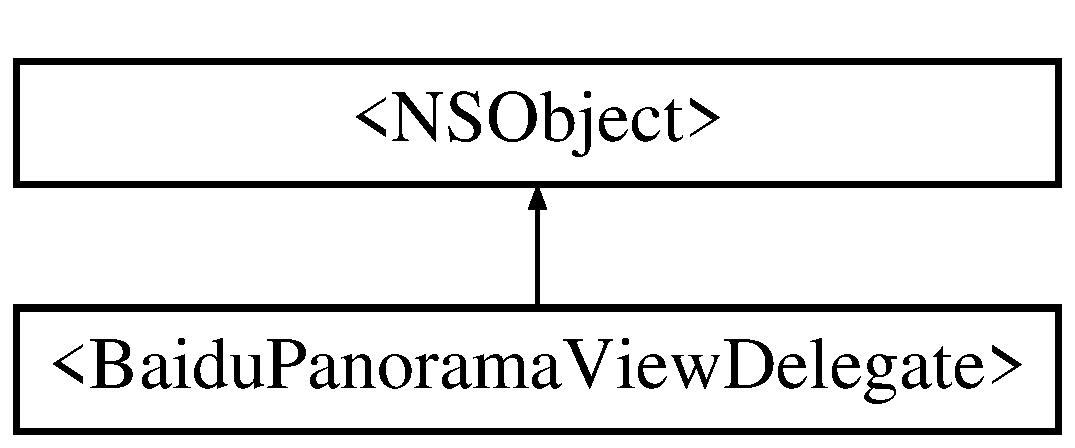
\includegraphics[height=2.000000cm]{protocol_baidu_panorama_view_delegate-p}
\end{center}
\end{figure}
\subsection*{Instance Methods}
\begin{DoxyCompactItemize}
\item 
(void) -\/ \hyperlink{protocol_baidu_panorama_view_delegate-p_a03539810d751c9ba222b787f77220634}{panorama\+Will\+Load\+:}
\item 
(void) -\/ \hyperlink{protocol_baidu_panorama_view_delegate-p_a24f54de59de8a2cdb3ee4671c1f79d73}{panorama\+Did\+Load\+:descreption\+:}
\item 
(void) -\/ \hyperlink{protocol_baidu_panorama_view_delegate-p_a4078254b3540500fc14b2f718ede1142}{panorama\+Load\+Failed\+:error\+:}
\item 
(void) -\/ \hyperlink{protocol_baidu_panorama_view_delegate-p_af45938530cd3b0e4c0309785c339af17}{panorama\+View\+:overlay\+Clicked\+:}
\end{DoxyCompactItemize}


\subsection{Method Documentation}
\hypertarget{protocol_baidu_panorama_view_delegate-p_a24f54de59de8a2cdb3ee4671c1f79d73}{}\index{Baidu\+Panorama\+View\+Delegate-\/p@{Baidu\+Panorama\+View\+Delegate-\/p}!panorama\+Did\+Load\+:descreption\+:@{panorama\+Did\+Load\+:descreption\+:}}
\index{panorama\+Did\+Load\+:descreption\+:@{panorama\+Did\+Load\+:descreption\+:}!Baidu\+Panorama\+View\+Delegate-\/p@{Baidu\+Panorama\+View\+Delegate-\/p}}
\subsubsection[{panorama\+Did\+Load\+:descreption\+:}]{\setlength{\rightskip}{0pt plus 5cm}-\/ (void) panorama\+Did\+Load\+: 
\begin{DoxyParamCaption}
\item[{({\bf Baidu\+Panorama\+View} $\ast$)}]{panorama\+View}
\item[{descreption:(N\+S\+String $\ast$)}]{json\+Str}
\end{DoxyParamCaption}
\hspace{0.3cm}{\ttfamily [optional]}}\label{protocol_baidu_panorama_view_delegate-p_a24f54de59de8a2cdb3ee4671c1f79d73}
全景图加载完毕 
\begin{DoxyParams}{Parameters}
{\em panorama\+View} & 当前全景视图 \\
\hline
{\em json\+Str} & 全景单点信息 \\
\hline
\end{DoxyParams}
\hypertarget{protocol_baidu_panorama_view_delegate-p_a4078254b3540500fc14b2f718ede1142}{}\index{Baidu\+Panorama\+View\+Delegate-\/p@{Baidu\+Panorama\+View\+Delegate-\/p}!panorama\+Load\+Failed\+:error\+:@{panorama\+Load\+Failed\+:error\+:}}
\index{panorama\+Load\+Failed\+:error\+:@{panorama\+Load\+Failed\+:error\+:}!Baidu\+Panorama\+View\+Delegate-\/p@{Baidu\+Panorama\+View\+Delegate-\/p}}
\subsubsection[{panorama\+Load\+Failed\+:error\+:}]{\setlength{\rightskip}{0pt plus 5cm}-\/ (void) panorama\+Load\+Failed\+: 
\begin{DoxyParamCaption}
\item[{({\bf Baidu\+Panorama\+View} $\ast$)}]{panorama\+View}
\item[{error:(N\+S\+Error $\ast$)}]{error}
\end{DoxyParamCaption}
\hspace{0.3cm}{\ttfamily [optional]}}\label{protocol_baidu_panorama_view_delegate-p_a4078254b3540500fc14b2f718ede1142}
全景图加载失败 
\begin{DoxyParams}{Parameters}
{\em panorama\+View} & 当前全景视图 \\
\hline
{\em error} & 加载失败的返回信息 \\
\hline
\end{DoxyParams}
\hypertarget{protocol_baidu_panorama_view_delegate-p_af45938530cd3b0e4c0309785c339af17}{}\index{Baidu\+Panorama\+View\+Delegate-\/p@{Baidu\+Panorama\+View\+Delegate-\/p}!panorama\+View\+:overlay\+Clicked\+:@{panorama\+View\+:overlay\+Clicked\+:}}
\index{panorama\+View\+:overlay\+Clicked\+:@{panorama\+View\+:overlay\+Clicked\+:}!Baidu\+Panorama\+View\+Delegate-\/p@{Baidu\+Panorama\+View\+Delegate-\/p}}
\subsubsection[{panorama\+View\+:overlay\+Clicked\+:}]{\setlength{\rightskip}{0pt plus 5cm}-\/ (void) panorama\+View\+: 
\begin{DoxyParamCaption}
\item[{({\bf Baidu\+Panorama\+View} $\ast$)}]{panorama\+View}
\item[{overlayClicked:(N\+S\+String $\ast$)}]{overlay\+Id}
\end{DoxyParamCaption}
\hspace{0.3cm}{\ttfamily [optional]}}\label{protocol_baidu_panorama_view_delegate-p_af45938530cd3b0e4c0309785c339af17}
全景图中的覆盖物点击事件 
\begin{DoxyParams}{Parameters}
{\em overlay\+Id} & 覆盖物标识 \\
\hline
\end{DoxyParams}
\hypertarget{protocol_baidu_panorama_view_delegate-p_a03539810d751c9ba222b787f77220634}{}\index{Baidu\+Panorama\+View\+Delegate-\/p@{Baidu\+Panorama\+View\+Delegate-\/p}!panorama\+Will\+Load\+:@{panorama\+Will\+Load\+:}}
\index{panorama\+Will\+Load\+:@{panorama\+Will\+Load\+:}!Baidu\+Panorama\+View\+Delegate-\/p@{Baidu\+Panorama\+View\+Delegate-\/p}}
\subsubsection[{panorama\+Will\+Load\+:}]{\setlength{\rightskip}{0pt plus 5cm}-\/ (void) panorama\+Will\+Load\+: 
\begin{DoxyParamCaption}
\item[{({\bf Baidu\+Panorama\+View} $\ast$)}]{panorama\+View}
\end{DoxyParamCaption}
\hspace{0.3cm}{\ttfamily [optional]}}\label{protocol_baidu_panorama_view_delegate-p_a03539810d751c9ba222b787f77220634}
全景图将要加载 
\begin{DoxyParams}{Parameters}
{\em panorama\+View} & 当前全景视图 \\
\hline
\end{DoxyParams}


The documentation for this protocol was generated from the following file\+:\begin{DoxyCompactItemize}
\item 
Baidu\+Panorama\+View.\+h\end{DoxyCompactItemize}

\hypertarget{interface_baidu_pano_utils}{}\section{Baidu\+Pano\+Utils Class Reference}
\label{interface_baidu_pano_utils}\index{Baidu\+Pano\+Utils@{Baidu\+Pano\+Utils}}
Inheritance diagram for Baidu\+Pano\+Utils\+:\begin{figure}[H]
\begin{center}
\leavevmode
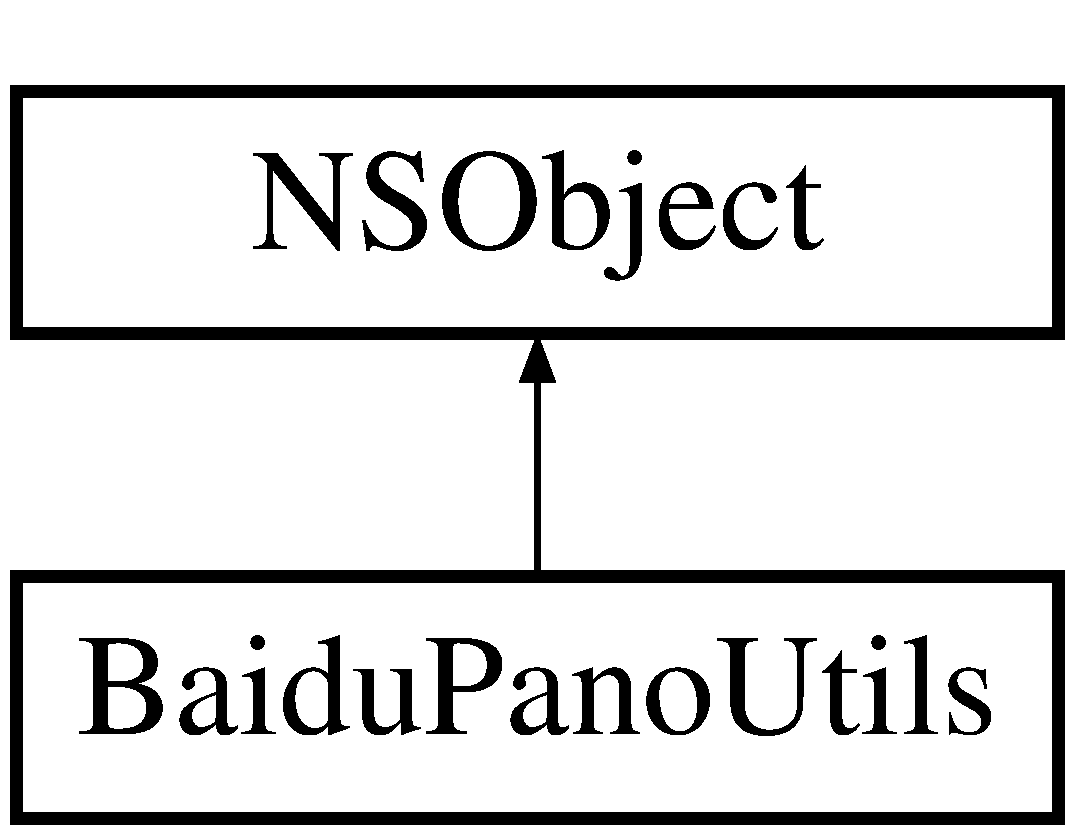
\includegraphics[height=2.000000cm]{interface_baidu_pano_utils}
\end{center}
\end{figure}
\subsection*{Class Methods}
\begin{DoxyCompactItemize}
\item 
(\hyperlink{struct_mecator_point}{M\+E\+C\+A\+T\+O\+R\+P\+O\+I\+N\+T}) + \hyperlink{interface_baidu_pano_utils_a139dfbfac5af14a0222611fe4eb50962}{get\+Mc\+With\+Lon\+:lat\+:}
\item 
(C\+L\+Location\+Coordinate2\+D) + \hyperlink{interface_baidu_pano_utils_a5e0a24b15903d8ad95cfb9ba4d09202b}{baidu\+Coor\+Encrypt\+Lon\+:lat\+:coor\+Type\+:}
\end{DoxyCompactItemize}


\subsection{Method Documentation}
\hypertarget{interface_baidu_pano_utils_a5e0a24b15903d8ad95cfb9ba4d09202b}{}\index{Baidu\+Pano\+Utils@{Baidu\+Pano\+Utils}!baidu\+Coor\+Encrypt\+Lon\+:lat\+:coor\+Type\+:@{baidu\+Coor\+Encrypt\+Lon\+:lat\+:coor\+Type\+:}}
\index{baidu\+Coor\+Encrypt\+Lon\+:lat\+:coor\+Type\+:@{baidu\+Coor\+Encrypt\+Lon\+:lat\+:coor\+Type\+:}!Baidu\+Pano\+Utils@{Baidu\+Pano\+Utils}}
\subsubsection[{baidu\+Coor\+Encrypt\+Lon\+:lat\+:coor\+Type\+:}]{\setlength{\rightskip}{0pt plus 5cm}+ (C\+L\+Location\+Coordinate2\+D) baidu\+Coor\+Encrypt\+Lon\+: 
\begin{DoxyParamCaption}
\item[{(double)}]{lon}
\item[{lat:(double)}]{lat}
\item[{coorType:(C\+O\+O\+R\+\_\+\+T\+Y\+P\+E)}]{type}
\end{DoxyParamCaption}
}\label{interface_baidu_pano_utils_a5e0a24b15903d8ad95cfb9ba4d09202b}
坐标转化工具,将其他坐标系的坐标转为百度坐标 
\begin{DoxyParams}{Parameters}
{\em lon:经度} & lat:纬度 type:其他坐标系类型 \\
\hline
\end{DoxyParams}
\hypertarget{interface_baidu_pano_utils_a139dfbfac5af14a0222611fe4eb50962}{}\index{Baidu\+Pano\+Utils@{Baidu\+Pano\+Utils}!get\+Mc\+With\+Lon\+:lat\+:@{get\+Mc\+With\+Lon\+:lat\+:}}
\index{get\+Mc\+With\+Lon\+:lat\+:@{get\+Mc\+With\+Lon\+:lat\+:}!Baidu\+Pano\+Utils@{Baidu\+Pano\+Utils}}
\subsubsection[{get\+Mc\+With\+Lon\+:lat\+:}]{\setlength{\rightskip}{0pt plus 5cm}+ ({\bf M\+E\+C\+A\+T\+O\+R\+P\+O\+I\+N\+T}) get\+Mc\+With\+Lon\+: 
\begin{DoxyParamCaption}
\item[{(double)}]{lon}
\item[{lat:(double)}]{lat}
\end{DoxyParamCaption}
}\label{interface_baidu_pano_utils_a139dfbfac5af14a0222611fe4eb50962}
百度地理坐标转化为百度墨卡托坐标 
\begin{DoxyParams}{Parameters}
{\em lon:经度} & lat:纬度 \\
\hline
\end{DoxyParams}


The documentation for this class was generated from the following file\+:\begin{DoxyCompactItemize}
\item 
Baidu\+Pano\+Utils.\+h\end{DoxyCompactItemize}

\hypertarget{interface_baidu_poi_pano_data}{}\section{Baidu\+Poi\+Pano\+Data Class Reference}
\label{interface_baidu_poi_pano_data}\index{Baidu\+Poi\+Pano\+Data@{Baidu\+Poi\+Pano\+Data}}
Inheritance diagram for Baidu\+Poi\+Pano\+Data\+:\begin{figure}[H]
\begin{center}
\leavevmode
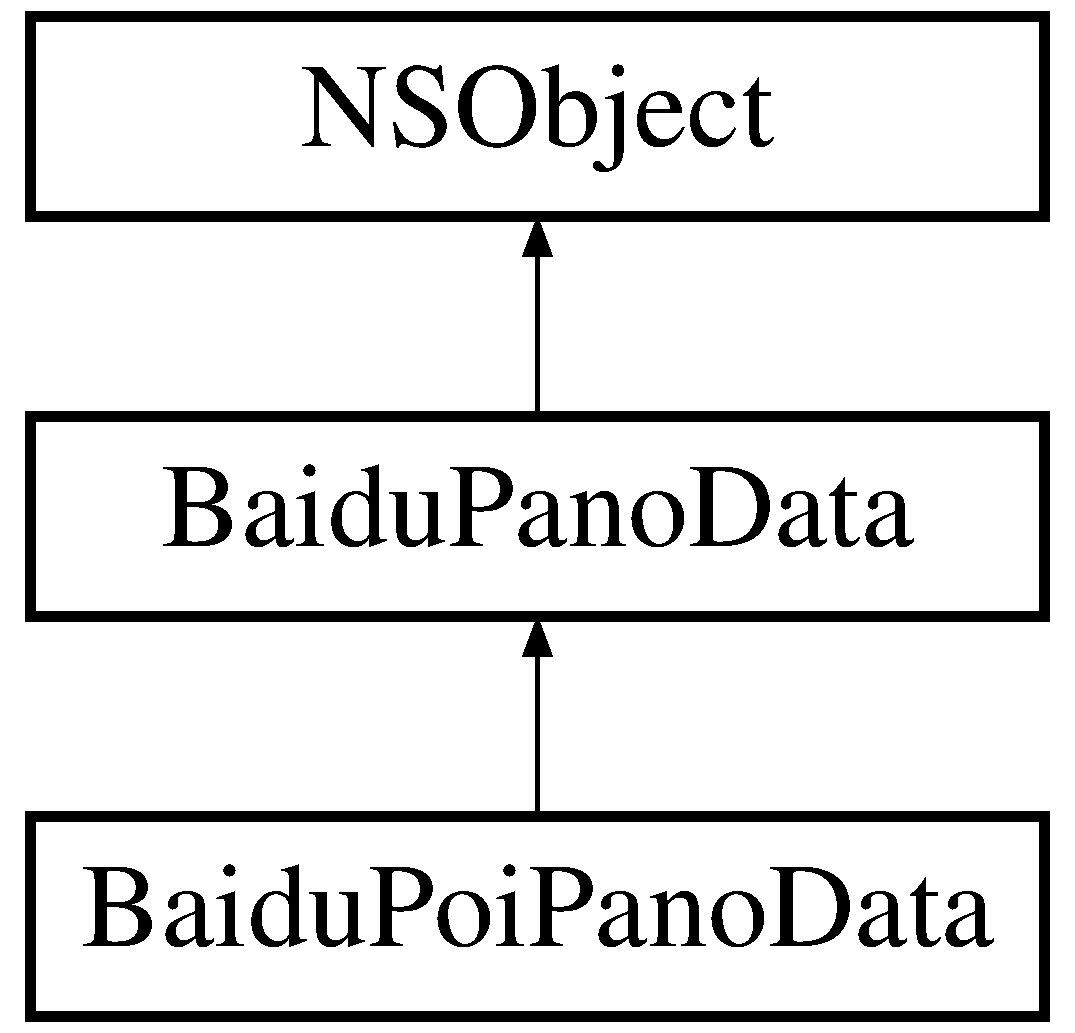
\includegraphics[height=3.000000cm]{interface_baidu_poi_pano_data}
\end{center}
\end{figure}
\subsection*{Properties}
\begin{DoxyCompactItemize}
\item 
\hypertarget{interface_baidu_poi_pano_data_a17c4b24a13ac5206d0748fe7048786ff}{}double {\bfseries direction}\label{interface_baidu_poi_pano_data_a17c4b24a13ac5206d0748fe7048786ff}

\item 
\hypertarget{interface_baidu_poi_pano_data_a4384437b74823a591e6ca9226ea38219}{}N\+S\+String $\ast$ {\bfseries pid}\label{interface_baidu_poi_pano_data_a4384437b74823a591e6ca9226ea38219}

\item 
\hypertarget{interface_baidu_poi_pano_data_a7b0c8edd5a8f85c9b9e31acf4e235a43}{}N\+S\+String $\ast$ {\bfseries uid}\label{interface_baidu_poi_pano_data_a7b0c8edd5a8f85c9b9e31acf4e235a43}

\item 
\hypertarget{interface_baidu_poi_pano_data_a125180d9df669dc673181c88fa021d0b}{}N\+S\+String $\ast$ {\bfseries iid}\label{interface_baidu_poi_pano_data_a125180d9df669dc673181c88fa021d0b}

\item 
\hypertarget{interface_baidu_poi_pano_data_aeb7c0130c5f013a37ff09a3f819713aa}{}N\+S\+String $\ast$ {\bfseries name}\label{interface_baidu_poi_pano_data_aeb7c0130c5f013a37ff09a3f819713aa}

\item 
\hypertarget{interface_baidu_poi_pano_data_a072afe529557cdede7eeaa41a61d082f}{}N\+S\+String $\ast$ {\bfseries std\+\_\+tag}\label{interface_baidu_poi_pano_data_a072afe529557cdede7eeaa41a61d082f}

\item 
\hypertarget{interface_baidu_poi_pano_data_a6b48d7057a5a8b779edb488712d9c1c8}{}B\+O\+O\+L {\bfseries has\+Street}\label{interface_baidu_poi_pano_data_a6b48d7057a5a8b779edb488712d9c1c8}

\item 
\hypertarget{interface_baidu_poi_pano_data_a36eaadc35ae42faf0e6fab9713b1fef5}{}B\+O\+O\+L {\bfseries has\+Interior}\label{interface_baidu_poi_pano_data_a36eaadc35ae42faf0e6fab9713b1fef5}

\end{DoxyCompactItemize}


The documentation for this class was generated from the following file\+:\begin{DoxyCompactItemize}
\item 
Baidu\+Poi\+Pano\+Data.\+h\end{DoxyCompactItemize}

\hypertarget{struct_mecator_point}{}\section{Mecator\+Point Struct Reference}
\label{struct_mecator_point}\index{Mecator\+Point@{Mecator\+Point}}
\subsection*{Public Member Functions}
\begin{DoxyCompactItemize}
\item 
\hypertarget{struct_mecator_point_a2a46e3fabd7ef447cb439b3be1292573}{}{\bfseries Mecator\+Point} (double dx, double dy)\label{struct_mecator_point_a2a46e3fabd7ef447cb439b3be1292573}

\end{DoxyCompactItemize}
\subsection*{Public Attributes}
\begin{DoxyCompactItemize}
\item 
\hypertarget{struct_mecator_point_a423ba8baedd3afab4f84621d001e59a8}{}double {\bfseries x}\label{struct_mecator_point_a423ba8baedd3afab4f84621d001e59a8}

\item 
\hypertarget{struct_mecator_point_a8d18558f7f9c4e8edf30d18761217574}{}double {\bfseries y}\label{struct_mecator_point_a8d18558f7f9c4e8edf30d18761217574}

\end{DoxyCompactItemize}


The documentation for this struct was generated from the following file\+:\begin{DoxyCompactItemize}
\item 
Baidu\+Pano\+Utils.\+h\end{DoxyCompactItemize}

%--- End generated contents ---

% Index
\backmatter
\newpage
\phantomsection
\clearemptydoublepage
\addcontentsline{toc}{chapter}{Index}
\printindex

\end{document}
